\documentclass{article}
\title{Using Makefiles and Version Control to Build Assignment}
\author{Daniel Wendt}

\usepackage{amsmath,amsthm,amssymb,graphicx,siunitx,float,listings,fullpage}

\begin{document}

\maketitle

\section{Makefiles and Version Control}

I used the makefile ``ph20makefile'' to build this pdf document, calling the code from the previous assignment to create the required plots and using the pdflatex command. The makefile also access and saves the git log recorded in this document. The text of this makefile is included below:

\subsection*{ph20makefile}
\texttt{\lstinputlisting[breaklines]{ph20makefile}}

Additionally, git was used to version control this assignment during the process of creating a makefile and modifying the code from the previous assignment. The version control log shows the process of changes, including my detour into making the code take command line input, and then deciding it was too hard to figure out how to plot multiple plots. Fortunately, the progress I made on this is saved using version control, so I may return to it someday. 

\pagebreak

\subsection*{git log}
\texttt{\lstinputlisting[breaklines]{textgitlog.txt}}

The python source code used is represented below. This program defines functions to create plots of different types of simulations of a harmonic oscillator, which are then called to plot and save the figures used in the second part of this assignment.

\subsection*{ph20numint2.py}
\texttt{\lstinputlisting[breaklines]{ph20numint2.py}}

\section{Numerical Model of Simple Harmonic Oscillator}

Numerical methods can be used to integrate and model systems involving differential equations, such as a simple harmonic oscillator like a mass on a spring. This system is described by Newton's second law and the spring equation: $$F=m\frac{d^2x}{dt^2}=-kx.$$ Using the explicit form of Euler's method of integrating differential equations, for a spring with mass and spring constant chosen so that $k=m$, we can derive $$x_{i+1}=x_i+hv_i,\quad v_{i+1}=v_i-hx_i.$$ I wrote a Python function to find the position and velocity of a spring over time given the input initial position and velocity, the number of points $N$ at which to find the value, and the interval $h$ between points. Figure \ref{eulerexplicit} shows the simulated approximation of position and velocity over time calculated for $x_0=1,v_0=0,N=4000,$ and $h=0.01$. This shows several cycles, demonstrating that the error inherent to this approximation causes the calculated amplitude of the oscillation to increase over time. 

\begin{figure}[H]
	\centering
	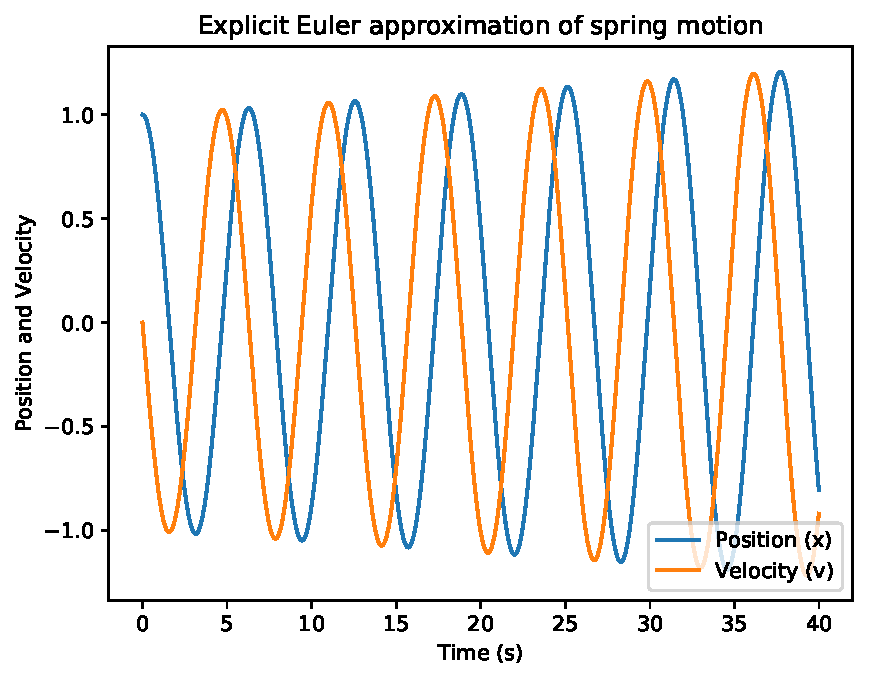
\includegraphics[width=0.6\textwidth]{eulerexplicit.pdf}
	\caption{A plot showing position and velocity over time for an explicit Euler method simulation of a harmonic oscillator. $N$ and $h$ have been chosen to show several cycles, with the amplitude increasing by a notable amount each cycle.}
	\label{eulerexplicit}
\end{figure}

The analytic solution to the system with these initial conditions is $$x=\cos(t),v=-\sin(t).$$ The error of this simulation can be analyzed by subtracting the analytic solution from the calculated solution. Figure \ref{expliciterror} shows the global error for several different values of $h$ up to the same final time, demonstrating that the error as a function of time is proportional to $h$. As $h$ increases by a factor of two, the error in $x$ and $v$ increases by a factor of two, with the error equaling zero when $x=0$ or $v=0$.

\begin{figure}[H]
	\centering
	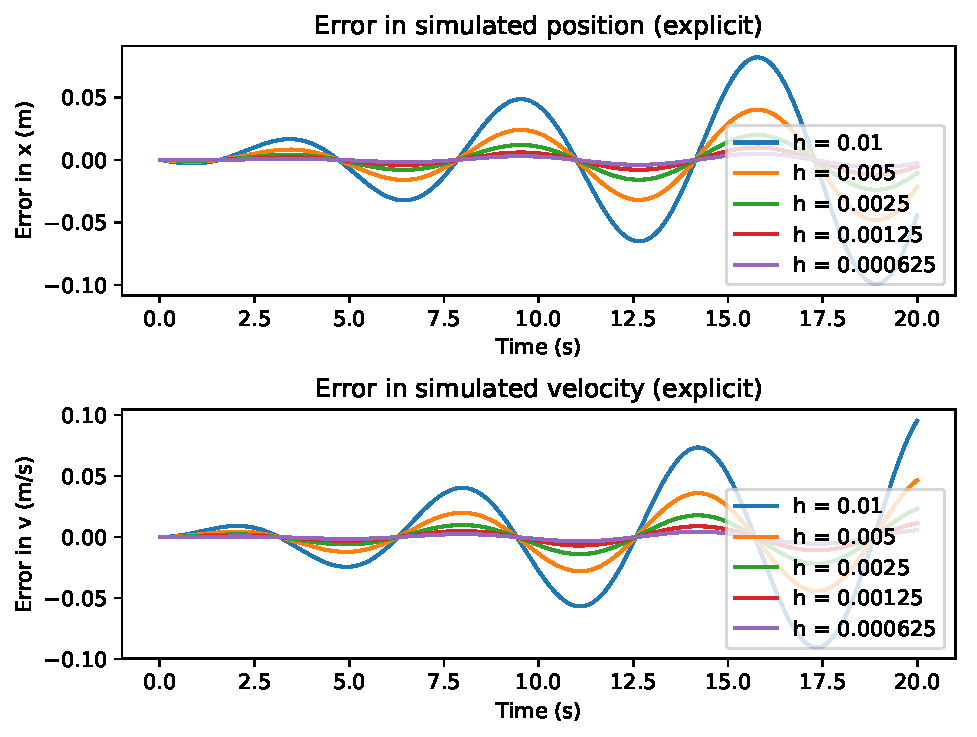
\includegraphics[width=0.6\textwidth]{eulerexpliciterror.pdf}
	\caption{A plot showing global error over time for position and velocity using the explicit Euler method of simulating a simple harmonic oscillator. The error is plotted for several different values of $h$, each increasing by a factor of 2.}
	\label{expliciterror}
\end{figure}

Because of the error in this simulation, the energy of the simulated system is not conserved. We can calculate the normalized total energy $E=x^2+v^2$ over time, which increases over time for the explicit Euler method as shown in Figure \ref{explicitenergy}. 

\begin{figure}[H]
	\centering
	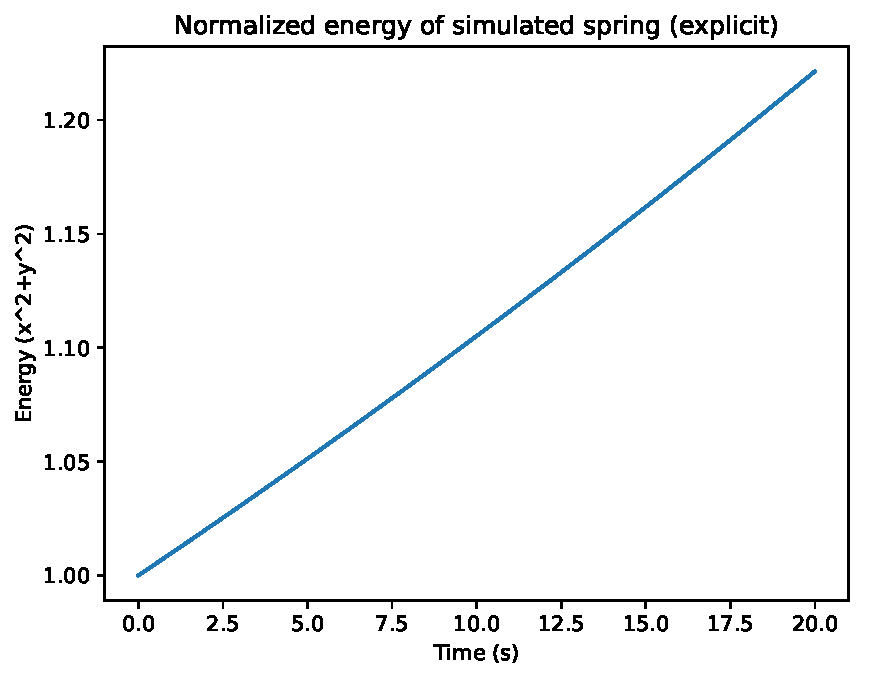
\includegraphics[width=0.6\textwidth]{eulerexplicitenergy.pdf}
	\caption{A plot showing normalized total energy over time for a harmonic oscillator simulated with the explicit Euler method. Over time, the energy increases approximately linearly, violating the conservation of energy expected for a real physical system.}
	\label{explicitenergy}
\end{figure}

The implicit Euler method uses the new position and velocity to compute the new position and velocity, rather than the old position and velocity. This gives the equations $$x_{i+1}=x_i+hv_{i+1},\quad v_{i+1}=v_i-hx_{i+1},$$ which can be solved to find $$x_{i+1}=\frac{x_i+hv_i}{1+h^2},\quad v_{i+1}=\frac{v_i-hx_i}{1+h^2}.$$ Using these equations, I simulated the same system with $x_0=1,v_0=0,N=4000,$ and $h=0.01$, plotted in Figure \ref{eulerimplicit}.

\begin{figure}[H]
	\centering
	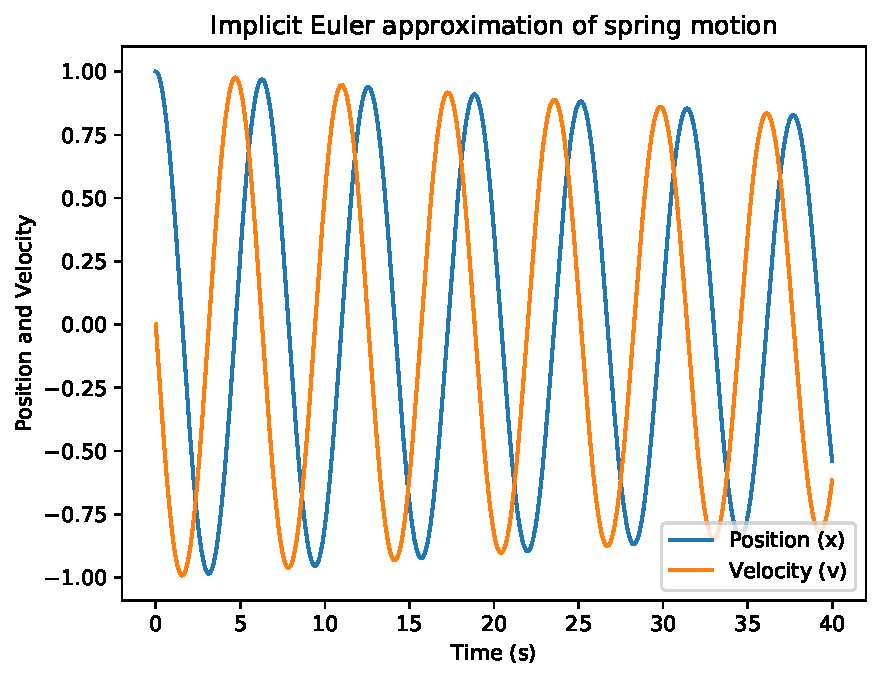
\includegraphics[width=0.6\textwidth]{eulerimplicit.pdf}
	\caption{A plot showing position and velocity over time for an explicit Euler method simulation of a harmonic oscillator. $N$ and $h$ have been chosen to show several cycles, with the amplitude decreasing by a notable amount each cycle, and the parameters the same as in Figure \ref{eulerexplicit}.}
	\label{eulerimplicit}
\end{figure}

I also plot the error and energy for the implicit Euler method, again using the same parameters as for the explicit method. These are shown in Figure \ref{impliciterror} and Figure \ref{implicitenergy} respectively. The error is still proportional to $h$, taking the same form as before with roughly the same amplitude over time for the same $h$, and the energy decreases approximately linearly over time.

\begin{figure}[H]
	\centering
	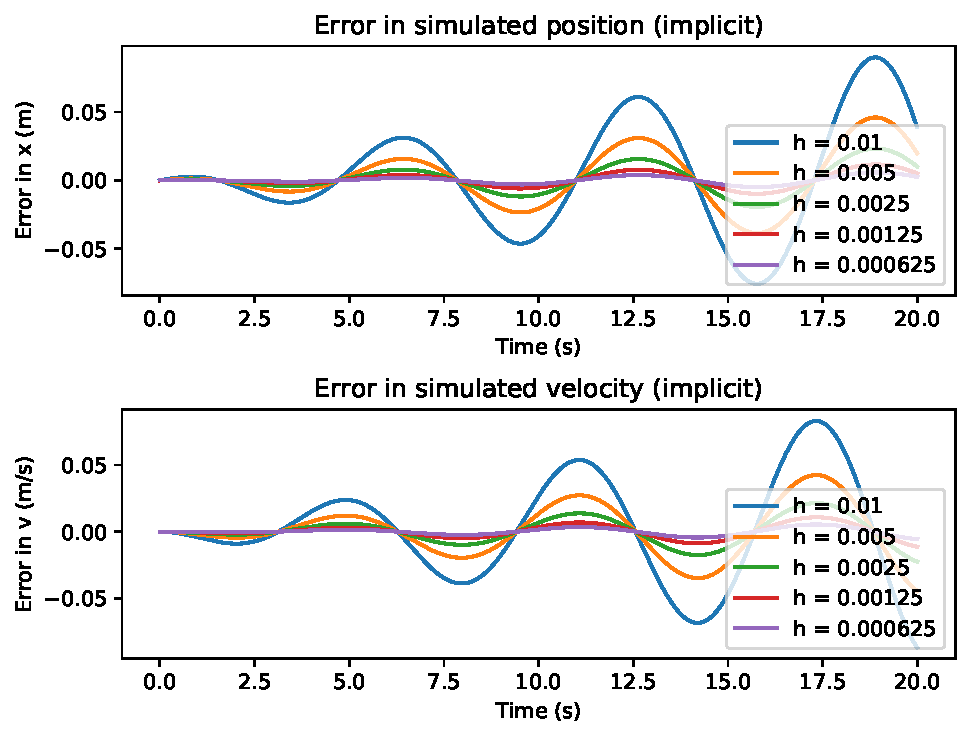
\includegraphics[width=0.6\textwidth]{eulerimpliciterror.pdf}
	\caption{A plot showing global error over time for position and velocity using the implicit Euler method of simulating a simple harmonic oscillator. The error is plotted for several different values of $h$, each increasing by a factor of 2.}
	\label{impliciterror}
\end{figure}

\begin{figure}[H]
	\centering
	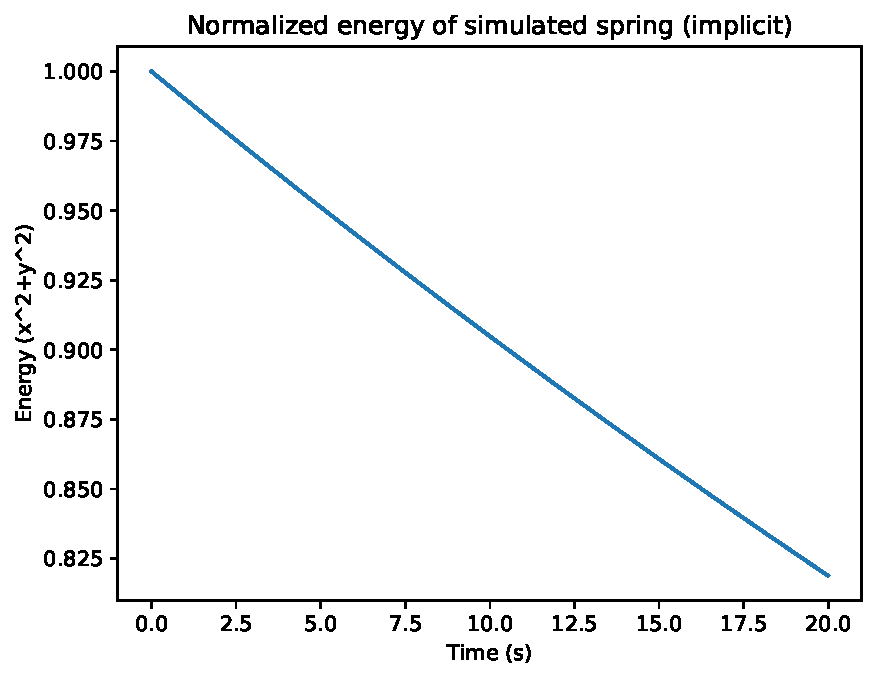
\includegraphics[width=0.6\textwidth]{eulerimplicitenergy.pdf}
	\caption{A plot showing normalized total energy over time for a harmonic oscillator simulated with the implicit Euler method. Over time, the energy decreases approximately linearly, similarly violating the conservation of energy expected for a real physical system, although in the opposite direction of the explicit method.}
	\label{implicitenergy}
\end{figure}

Phase space, as seen in Assignment 1, is a useful tool for analyzing the phase of oscillating systems. I have also plotted the results from the implicit and explicit Euler approximations in phase space, plotting $v$ against $x$. Figure \ref{phasespace} shows these plots and the expected analytic solution. These accumulate no phase error, with the increasing or decreasing amplitude causing a circular spiral outward or inward. 

\begin{figure}[H]
	\centering
	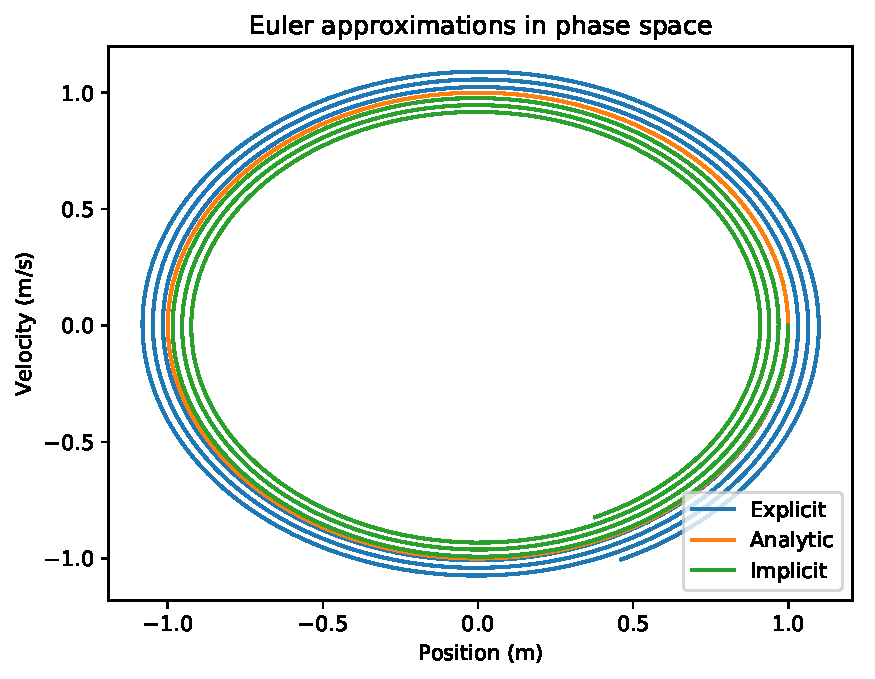
\includegraphics[width=0.6\textwidth]{eulerphasespace.pdf}
	\caption{A plot showing the phase-space geometry of the explicit and implicit Euler approximations, and the expected analytic solution. Each approximation has $x$ plotted against $v$. The explicit and implicit approximations spiral without changing phase as their amplitude increases or decreases over time.}
	\label{phasespace}
\end{figure}

Another method of approximating, the symplectic Euler method, conserves energy on the average much more effectively. This integrator uses the equations $$x_{i+1}=x_i+hv_i,\quad v_{i+1}=v_i-hx_{i+1}.$$ Figure \ref{phasesymp} shows this approximation in phase-space, for $h=0.2$, compared to the explicit Euler approximation with the same $h$ and the analytic solution. The symplectic approximation stays much closer to the analytic solution, but $x$ and $v$ become slightly out of phase with one another, as shown by the deformation of the symplectic ellipse from the analytic circle. 

\begin{figure}[H]
	\centering
	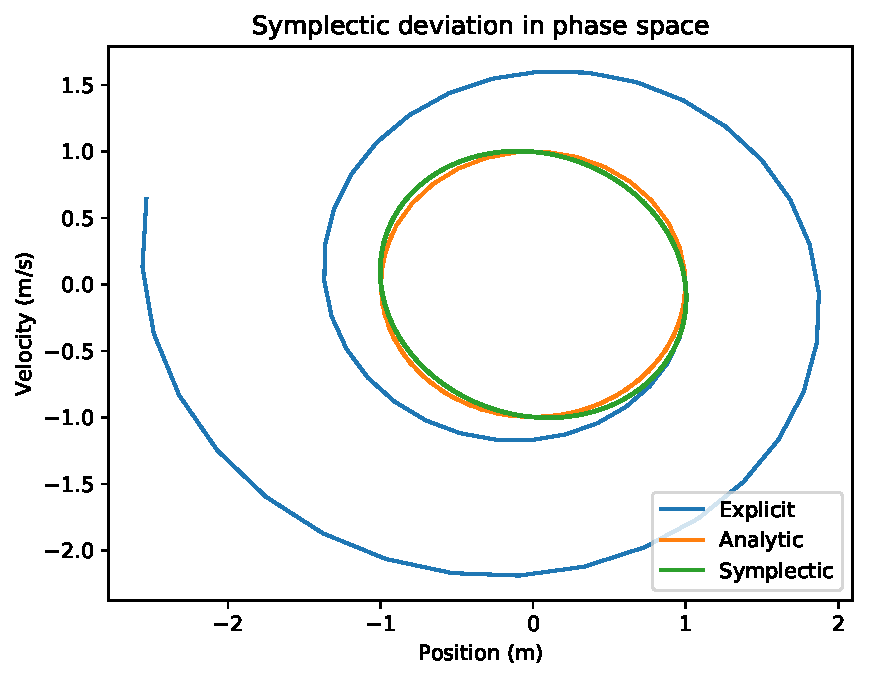
\includegraphics[width=0.6\textwidth]{eulerphasesymp.pdf}
	\caption{A plot showing the phase-space geometry of the symplectic and explicit Euler approximations, and the expected analytic solution. Each approximation has $x$ plotted against $v$. While the explicit solution spirals outward, the symplectic solution remains close to the analytic solution, but slightly out of phase.}
	\label{phasesymp}
\end{figure}

The error in the phase of this approximation shows up in the average energy calculated by the symplectic Euler method. The normalized total energy, calculated like with the previous approximations, is plotted in Figure \ref{sympenergy}. Unlike the explicit and implicit Euler methods, the symplectic energy is sinusoidal, oscillating around the expected central value of 1. This corresponds to the phase-space diagram, where the symplectic approximation deviated slightly from the circle of $x^2+v^2=E$, repeatedly cycling between lower and higher. 

\begin{figure}[H]
	\centering
	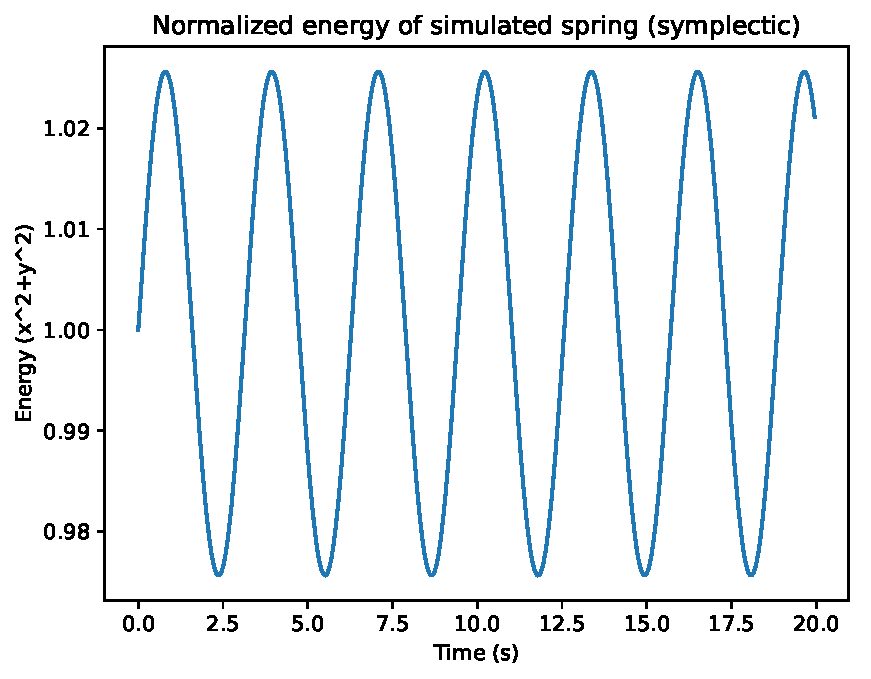
\includegraphics[width=0.6\textwidth]{eulersymplecticenergy.pdf}
	\caption{A plot showing the phase-space geometry of the explicit and implicit Euler approximations, and the expected analytic solution. Each approximation has $x$ plotted against $v$. The explicit and implicit approximations spiral without changing phase as their amplitude increases or decreases over time.}
	\label{sympenergy}
\end{figure}

Since the average energy is conserved, this makes the symplectic method more attractive for approximating this physical system. However, this method does introduce the phase error, so it is not perfect.

\end{document}
